\chapter{New contributions}


\section{Algorithmic approach}
\label{sec:algo_approach}

There are $2$ intuitive ways to tackle the problem of the Krenn's conjecture.
The first way is to use an algorithmic approach to find interesting properties about perfectly monochromatic graphs.
In this approach, I hope that the conjecture is true and try to prove it in some very restricted cases.
This is what is done in this section.\\

The second approach is a computational approach.
Its interests and realisation are discussed in section~\ref{sec:computational_approach}.

\subsection{Problem reduction}
\label{subsec:problem_reduction}

\subsection{Constraints relaxation}
\label{subsec:constraints_relaxation}

As it was explained in the introduction, a simplified version of the conjecture was already proven thanks to Bogdanov.\cite{bogdanov}
This version, presented in lemma~\ref{lem:real_pos_weights}, is only valid when all the weights of a perfectly monochromatic graph $G_k^w$ are positive.
In this section, our main goal will be to relax these constraints.

\subsubsection{Allowing one negative edge}
\label{subsubsec:one_negative_edge}

Since the conjecture is proven to be true when all the weights are positive, it is natural to ask ourselves how the proof would be affected if this constraint was relaxed.
The most simple case is the one where one edge is allowed to have a negative weight.
The goal of this section is to answer that question.

\begin{observation}[Existence of a Hamiltonian cycle]
    \label{obs:one_neg_edge_ham_cycle}
    Let $G_k^w$ be a simple perfectly monochromatic graph that has only real weights, and that has exactly one edge $e^-$ whose weight is negative.
    If $\Tilde{c}(G, k, w) \geq 3$, then the graph has $3$ monochromatic perfect matchings $M_1, M_2$ and $M_3$ of colour $1$, $2$ and $3$ respectively.
    Assuming that the colour of $e^-$ is $3$, then the union of $M_1$ and $M_2$ forms a Hamiltonian cycle of even length.
\end{observation}

\begin{proof}
    Since $M_1$ and $M_2$ are disjoint, they form a disjoint union of $\mathcal{C}$ cycles of even length.
    If $\mathcal{C} \geq 2$, we will denote by $C_i$ the $i^{th}$ cycle.
    Then, we can build the following non-monochromatic perfect matching :

    \begin{center}
        $N = (C_1 \cap M_1) \cup (\bigcup\limits_{i=2}^{\mathcal{C}} C_i \cap M_2)$
    \end{center}

    The construction of $N$ is represented in figure~\ref{fig:proof_unique_neg_ham}.

    \begin{figure}[H]
        \ctikzfig{figures/new_results/unique_neg/unique_neg_ham}
        \caption{In this example, the non-monochromatic perfect matching $N$ (represented by thick edges) is constructed from a red PM and a green PM. The induced vertex colouring is also visible.}
        \label{fig:proof_unique_neg_ham}
    \end{figure}

    Since $M_1$ and $M_2$ include no negatively weighted edge, $w(N) > 0$.
    But, by definition~\ref{def:perfectly_monochromatic_graph} of a perfectly monochromatic graph, and using the notations introduced in definitions \ref{def:matching_weight} and \ref{def:feasible_vertex_colouring},

    \begin{center}
        $w(\kappa(N)) = \sum\limits_{N_i \in \mathcal{M}_{\kappa(N)}} N_i = 0$
    \end{center}

    Therefore, we know that $\exists N'$ such that $\kappa(N') = \kappa(N)$ and $w(N') < 0$. This is impossible, because the only way for $N'$ to have a negative weight is to include $e^-$, which has colour $3 \neq 1$ nor $2$. The conclusion is that $\mathcal{C} = 1$, which means that $M_1$ and $M_2$ form a Hamiltonian cycle.
\end{proof}


\begin{observation}[Parity of crossing edges]
    \label{obs:one_neg_edge_parity_crossing_edges}
    Let $G_k^w$ be a simple perfectly monochromatic graph that has only real weights, and that has exactly one edge $e^-$ who's weight is negative. If $\Tilde{c}(G, k, w) \geq 3$, then the graph has $3$ monochromatic perfect matchings $M_1, M_2$ and $M_3$ of colour $1$, $2$ and $3$ respectively. Assuming that the colour of $e^-$ is $3$, let $H = (v_1, \dots, v_n)$ be the Hamiltonian cycle of $G_k^w$ formed by $M_1$ and $M_2$. Let $e = (v_i, v_j)$ be an edge who's colour is $3$. Then $j-i$ is even.
\end{observation}

\begin{proof}
    Let assume by contradiction that $j-i$ is odd. Without loss of generality, we can assume that the colour of $(v_i, v_{i+1})$ is $1$ (otherwise, inverse colours $1$ and $2$ in the following reasoning). Using the notation introduced in definition \ref{def:arc}, we can build the following non-monochromatic perfect matching

    \begin{center}
        $N = e \cup (M_2 \cap H_{i+1, j-1}) \cup (M_1 \cap H_{j+1, i-1})$
    \end{center}

    The construction of the non-monochromatic perfect matching $N$ is represented in figure \ref{fig:unique_neg_odd_crossings}.

    \begin{figure}[H]
        \ctikzfig{figures/new_results/unique_neg/unique_neg_odd_crossings}
        \caption{Construction of $N$ from $M_1$, $M_2$ and $e$ if $j-i$ is odd.}
        \label{fig:unique_neg_odd_crossings}
    \end{figure}

    \begin{itemize}
        \item If $e \neq e^-$, then $w(N) > 0$. Therefore $\exists$ another non-monochromatic perfect matching $N'$ such that $\kappa(N') = \kappa(N)$ and $w(N') < 0$. To satisfy this constraint, $e^- \in N'$. This is impossible, because $e^- \neq (v_i, v_j)$, and these are the only vertices that get colour $3$ in $\kappa(N)$.

        \item If $e = e^-$, then $w(N) < 0$. Therefore $\exists$ another non-monochromatic perfect matching $N'$ such that $\kappa(N') = \kappa(N)$ and $w(N') > 0$. To satisfy this constraint, $e^- \notin N'$. This is impossible, because $e^- = (v_i, v_j)$, and these are the only vertices that get colour $3$ in $\kappa(N)$.
    \end{itemize}
\end{proof}

These observation may seem obscure at first, but they are necessary to prove the following lemma.

\begin{lemma}[One negative edge allowed]
    \label{lem:one_neg_edge}
    Let $G_k^w$ be a simple perfectly monochromatic graph that has only real weights, and that has maximum one edge who's weight is negative. Then, if $G$ is not isomorphic to $K_4$, $\Tilde{c}(G, k, w) \leq 2$.
\end{lemma}

The sketch of the proof of lemma \ref{lem:one_neg_edge} goes as follow. Using observations \ref{obs:one_neg_edge_ham_cycle} and \ref{obs:one_neg_edge_parity_crossing_edges}, we build a Hamiltonian cycle that has 2 colours and build non-monochromatic perfect matchings in it that use a negative edge $e$. We then show that they create a disbalance in the weight of their feasible vertex colouring that can not be counterbalanced with another perfect matching. Let's dive into it.

\begin{proof}[Proof of lemma \ref{lem:one_neg_edge}]

    Let $G_k^w$ be a simple perfectly monochromatic graph that has only real weights, and that has maximum one edge who's weight is negative. Let assume by contradiction that the weighted matching index of $G_k^w$ $\Tilde{c}(G, k, w)$ is $3$.

    \begin{enumerate}
        \item[]

        \item If $G_k^w$ has only positive weights, then we're done - this case is already solved.

        \item If $G_k^w$ has exactly one negative weight : let $M_1$, $M_2$ and $M_3$ be 3 distinct monochromatic perfect matchings of $G_k^w$ that have colour $1$, $2$ and $3$ respectively. They exist by definition \ref{def:weighted_matching_index} of the weighted matching index. Let $e^-$ be the only negatively weighted edge of $G_k^w$. Without loss of generality, I will say that the colour of $e^-$ is $3$. From observation \ref{obs:one_neg_edge_ham_cycle}, $M_1$ and $M_2$ form a Hamiltonian cycle $H = (v_1, v_2, \dots, v_n)$ of even length. In this new vertex ordering, $e^- = (v_i, v_j)$. We know from observation \ref{obs:one_neg_edge_parity_crossing_edges} that $j-i$ is even. Without loss of generality, I can assume that the color of $(v_i, v_{i + 1})$ is $1$ (otherwise we exchange colours $1$ and $2$ in the following reasoning). Let $e = (v_{i + 1}, v_k) \in M_3$ (we are certain of the existence of $e$ because $v_{i+1}$ must be covered by $M_3$). Now, $3$ situations can occur.

        \begin{enumerate}
            \item if $v_k = v_j$ : this situation is impossible from observation \ref{obs:one_neg_edge_parity_crossing_edges}, because $k - (i + 1)$ is odd.

            \item if $v_k$ appears in an edge from $P_{j+1, i-1}(H)$, then we can form a non-monochromatic perfect matching as follow.

            \begin{center}
                $N = \{e^-, e\} \cup (H_{j+1, k-1} \cap M_2) \cup (H_{i + 2, j - 1} \cap M_1) \cup (H_{k+1, i-1} \cap M_1)$
            \end{center}

            This works because we are sure that $k - (i + 1)$ is even from observation \ref{obs:one_neg_edge_parity_crossing_edges}. Since $e^- \in N$, $w(N) < 0$. But $w(\kappa(N)) = 0$ by definition of a perfectly monochromatic graph. Therefore, $\exists$ a non-monochromatic perfect matching $N'$ such that $\kappa(N') = \kappa(N)$ and $w(N') > 0$. This is possible only if $e^- \notin N'$. The only vertices that get colour $3$ in $\kappa(N) = \kappa(N')$ are $v_i, v_{i+1}, v_j$ and $v_k$. The only way to match these vertices in $N'$ with $3$-coloured edges without using $e^-$ is that $\exists e' = (v_i, v_k)$ and $e'' = (v_{i+1}, v_j)$ that have colour $3$ and that are included in $N'$. But this is impossible, because $k-i$ and $j-(i+1)$ are odd numbers, which is forbidden by observation \ref{obs:one_neg_edge_parity_crossing_edges}.

            \begin{figure}[H]
                \ctikzfig{figures/new_results/unique_neg/unique_neg_2_2}
                \caption{Illustration of the reasoning in case 2.2. In this figure, $N$ is represented by thick edges, and the induced vertex colouring from $N$ is visible. The edges $e'$ and $e''$ that should be in $N'$ are also represented. It is clear in this figure that $e'$ and $e''$ can't exist using the parity argument.}
                \label{fig:unique_neg_2_2}
            \end{figure}

            \item if $v_k$ appears in an edge from $H_{i+1, j-1}$, then it is possible to find an edge of $M_3$, called $e' = (v_l, v_m)$, that has both endpoint in $H_{i+1, k}(H)$, and such that the edge $e'' = (v_{l+1}, v_n) \in M_3$ has its $v_n$-endpoint in $H_{m+1, l-1}(H)$. This is true because it is known from observation \ref{obs:one_neg_edge_parity_crossing_edges} that $m-l$ is even. Actually, $e'$ might be equal to $e$. Assuming without loss of generality that the colour of $(v_l, v_{l+1})$ is $1$, we find a new non-monochromatic perfect matching

            \begin{center}
                $N = \{e', e''\} \cup (H_{l+2, m-1} \cap M_1) \cup (H_{n+1, l-1} \cap M_1) \cup (H_{m+1, n-1} \cap M_2)$
            \end{center}

            \begin{figure}[H]
                \ctikzfig{figures/new_results/unique_neg/unique_neg_2_3}
                \caption{Illustration of the reasoning in case 2.3. In this figure, $N$ is represented by thick edges, and the induced vertex colouring from $N$ is visible. It this particular case, $v_j = v_n$. Nevertheless, it is impossible for $v_i$ and $v_j$ to be both green in $\kappa(N)$.}
                \label{fig:unique_neg_2_3}
            \end{figure}

            Since $e^- \notin N$, $w(N) > 0$. But $w(\kappa(N)) = 0$ by definition of a perfectly monochromatic graph. Therefore, $\exists$ another non-monochromatic perfect matching $N'$ such that $\kappa(N') = \kappa(N)$ and $w(N') < 0$. For this condition to be satisfied, $e^- \in N'$. But it is impossible that both $v_i$ and $v_j$ get colour $3$ in $\kappa(N) = \kappa(N')$ (only one of them maximum). This means that $e^-$ can't be in $N'$, which forms a contradiction.
        \end{enumerate}
    \end{enumerate}

\end{proof}

\subsubsection{Allowing an arbitrary number of negative weights in one single colour class}

The main argument of the proof of the previous analysed case was that 2 colour classes had only positive weighted edges. This suggests that the structure of the proof might work as well if more than one single negatively weighted edge was present in the combination of the other colour classes. Such a result would be even more powerful since it would prove the conjecture to be true whenever 2 colour classes have only positive weighted edges, no matther the weights of the other colour classes. In this section, we will reuse the arguments from section \ref{subsubsec:one_negative_edge} to verify them in the situation where multiple negative edge weights are allowed.

\begin{observation}[Existence of a Hamiltonian cycle]
    \label{obs:2_positive_classes_ham_cycle}
    Let $G_k^w$ be a simple perfectly monochromatic graph that has only real weights, and that has exactly at least 2 colour classes that have only positive weights. If $\Tilde{c}(G, k, w) \geq 3$, then the graph has $3$ monochromatic perfect matchings $M_1, M_2$ and $M_3$ of colour $1$, $2$ and $3$ respectively. Assuming that $M_1$ and $M_2$ have only positive edges, then the union of $M_1$ and $M_2$ forms a Hamiltonian cycle of even length.
\end{observation}

\begin{proof}
    Since $M_1$ and $M_2$ are disjoint, they form a disjoint union of $\mathcal{C}$ cycles of even length. If $\mathcal{C} \geq 2$, we will denote by $C_i$ the $i^{th}$ cycle. Then, we can build the following non-monochromatic perfect matching :
    \begin{center}
        $N = (C_1 \cap M_1) \cup (\bigcup\limits_{i=2}^{\mathcal{C}} C_i \cap M_2)$
    \end{center}

    The construction of $N$ is highlighted in figure \ref{fig:demo_unique_neg_ham}.

    \begin{figure}[H]
        \ctikzfig{figures/new_results/2_pos_classes/2_pos_classes_ham_cycle}
        \caption{In this example, the non-monochromatic perfect matching $N$ (represented by thick edges) is constructed from a red perfect matching and a blue one. The induced vertex colouring is also visible.}
        \label{fig:demo_unique_neg_ham}
    \end{figure}

    Since $M_1$ and $M_2$ include no negatively weighted edge, $w(N) > 0$. But, by definition \ref{def:perfectly_monochromatic_graph} of a perfectly monochromatic graph, and using the notations introduced in definitions \ref{def:matching_weight} and \ref{def:feasible_vertex_colouring},

    \begin{center}
        $w(\kappa(N)) = \sum\limits_{N_i \in \mathcal{M}_{\kappa(N)}} N_i = 0$
    \end{center}

    Therefore, we know that $\exists N'$ such that $\kappa(N') = \kappa(N)$ and $w(N') < 0$. This is impossible, because the only way for $N'$ to have a negative weight is to include at least one negative edge. And negative edges don't exist in colour $1$ nor $2$. We can conclude that $\mathcal{C} = 1$, which means that $M_1$ and $M_2$ form a Hamiltonian cycle.
\end{proof}

\begin{observation}[Parity of crossing edges]
    \label{obs:2_positive_classes_parity_crossing_edge}
    Let $G_k^w$ be a simple perfectly monochromatic graph that has only real weights, and that has at least $2$ colour classes that have only positive weights. If $\Tilde{c}(G, k, w) \geq 3$, then the graph has $3$ monochromatic perfect matchings $M_1, M_2$ and $M_3$ of colour $1$, $2$ and $3$ respectively. Assuming that the colour classes $1$ and $2$ have only positive edges, let $H = (v_1, \dots, v_n)$ be the Hamiltonian cycle of $G_k^w$ formed by $M_1$ and $M_2$. Let $e = (v_i, v_j)$ be an edge who's colour is $3$. Then $j-i$ is even.
\end{observation}

\begin{proof}
    Let assume by contradiction that $j-i$ is odd. Without loss of generality, we can assume that the colour of $(v_i, v_{i+1})$ is $1$ (otherwise, inverse colours $1$ and $2$). Then the following non-monochromatic perfect matching can be built.

    \begin{center}
        $N = e \cup (M_2 \cap H_{i+1, j-1}) \cup (M_1 \cap H_{j+1, i-1})$
    \end{center}

    The construction of the non-monochromatic perfect matching $N$ is shown in figure \ref{fig:2_pos_classes_odd_crossings}.

    \begin{figure}[H]
        \ctikzfig{figures/new_results/unique_neg/unique_neg_odd_crossings}
        \caption{Construction of $N$ from $M_1$, $M_2$ and $e$ if $j-i$ is odd.}
        \label{fig:2_pos_classes_odd_crossings}
    \end{figure}

    \begin{itemize}
        \item If $w(e) > 0$, then $w(N) > 0$. Therefore $\exists$ another non-monochromatic perfect matching $N'$ such that $\kappa(N') = \kappa(N)$ and $w(N') < 0$. To satisfy this constraint, $e \in N'$. But $e$ is the only edge that has a colour different from $1$ nor $2$ in $N'$, which means that the sign of $w(e)$ determines the sign of $w(N')$. Therefore, $w(N')$ can not be negative. This is a contradiction.

        \item If $w(e) < 0$, then $w(N) < 0$. Therefore $\exists$ another non-monochromatic perfect matching $N'$ such that $\kappa(N') = \kappa(N)$ and $w(N') > 0$. To satisfy this constraint, $e \in N'$. But $e$ is the only edge that has a colour different from $1$ nor $2$ in $N'$, which means that the sign of $w(e)$ determines the sign of $w(N')$. Therefore, $w(N')$ can not be positive. This is also a contradiction, and ends the proof.
    \end{itemize}
\end{proof}

Now that we have verified that the two observations made in the previous section still hold in this section, let's extend our constraint relaxation by allowing every class except 2 of them to have an arbitrary number of negatively weighted edges.

\begin{lemma}[2 positive colour classes]
    \label{lem:2_positive_colour_classes_forbidden}
    Let $G_k^w$ be a simple perfectly monochromatic graph that has only real weights, and that has at least $2$ colour classes that have only positive weighted edges. Then, if $G$ is not isomorphic to $K_4$, $\Tilde{c}(G, k, w) \leq 2$.
\end{lemma}

\begin{proof}
    Let $M_1$, $M_2$ and $M_3$ be 3 distinct monochromatic perfect matchings of $G_k^w$ that have colour $1$, $2$ and $3$ respectively, and let assume that the colour classes $1$ and $2$ have only positive weighted edges. From observation \ref{obs:2_positive_classes_ham_cycle}, $M_1$ and $M_2$ form a Hamiltonian cycle $H = (v_1, v_2, \dots, v_n)$ of even length. We know from observation \ref{obs:2_positive_classes_parity_crossing_edge} that $\forall e = (v_i, v_j) \in M_3$, $j-i$ is even. Without loss of generality, let's assume that the color of $(v_i, v_{i + 1})$ is $1$ (otherwise we exchange colours $1$ and $2$). Let $e = (v_i, v_j) \in M_3$ be a minimal crossing edge, i.e. be such that $e' = (v_{i+1}, v_k) \in M_3$ has its $v_k$ endpoint in $P_{j+1, i-1}$. It is then possible to find a non-monochromatic perfect matching as follow.

    \begin{center}
        $\begin{array}{r c l}
             N & = & e                             \\
             &   & \cup e'                       \\
             &   & \cup M_1 \cap P_{i+2, j-1}(H) \\
             &   & \cup M_1 \cap P_{k+1, i-1}(H) \\
             &   & \cup M_2 \cap P_{j+1, k-1}(H)
        \end{array}$
    \end{center}

    The construction of $N$ is visualized in figure \ref{fig:2_pos_classes_proof}.

    \begin{figure}[H]
        \ctikzfig{figures/new_results/2_pos_classes/2_pos_classes_proof}
        \caption{Construction of $N$ from $M_1$, $M_2$, $e$ and $e'$. $N$ is represented by the thick edges. $\kappa(N)$ is also represented.}
        \label{fig:2_pos_classes_proof}
    \end{figure}

    Centering the analysis around the potential signs of $w(e)$ and $w(e')$, $2$ situations can occur.

    \begin{enumerate}
        \item if $w(e)$ and $w(e')$ have the same sign : then $w(N) > 0$. This means that $\exists N'$ such that $\kappa(N') = \kappa(N)$ and $w(N') < 0$. Since the sign of $N'$ is defined by the sign of its $3$-coloured edges, this last condition is satisfied only if $\exists e'' = (v_i, v_k)$ and $e''' = (v_{i+1}, v_j)$ of colour $3$. But this is forbidden by observation \ref{obs:2_positive_classes_parity_crossing_edge} because $k - i$ (and $j - (i + 1)$) is odd.

        \item if $w(e)$ and $w(e')$ have a different sign : then $w(N) < 0$. This means that $\exists N'$ such that $\kappa(N') = \kappa(N)$ and $w(N') > 0$. Since the sign of $N'$ is defined by the sign of its $3$-coloured edges, this last condition is satisfied only if $\exists e'' = (v_i, v_k)$ and $e''' = (v_{i+1}, v_j)$ of colour $3$. But this is forbidden by observation \ref{obs:2_positive_classes_parity_crossing_edge} because $k - i$ (and $j - (i + 1)$) is odd. This ends the proof of lemma \ref{lem:2_positive_colour_classes_forbidden}.
    \end{enumerate}

\end{proof}


\section{Computational approach}
\label{sec:computational_approach}

In order to find a counter example to the Krenn's conjecture in the best case scenario, or just to find interesting new properties in perfectly monochromatic graphs, having a more experimental approach has many interests. In this section, I am introducing a new tool I developped, called EGPI, that computes the weighted matching index of experiment graphs. Then, some of its potential uses are presented.

\subsection{Motivation}
\label{sec:computational_motivations}

Finding interesting examples of experimental graphs to study can be challenging due to the high degree of freedom experiment graphs can have, by definition \ref{def:experiment_graph}. Also, the weighted matching index of experiment graphs as defined in definition \ref{def:weighted_matching_index} is hard to find by hand since it requires to find all perfect matchings of a graph. In my knowledge, no public access tool exists at the time of the writing to easily encode experimental graphs and compute their weighted matching index. My hope is that such a tool could help me and other researchers to quickly verify some properties on instances of graphs they want to test, without losing more time on it. For this reason, I developed a new program that does exactly that. The program is called \textbf{EGPI}, which stands for \textbf{Experiment Graphs Properties Identifier}. I believe this name resumes the whole meaning of its utilisation.

\subsection{Functionalities of EGPI}

At the current state of its development, EGPI allows the user to do the following :

\begin{enumerate}
    \item \textbf{Discover all the perfect matchings of an encoded experiment graph}. The perfect matchings are encoded as edges sets. Their encoding includes an access to their weights and to the feasible vertex colouring they induce.
    \item \textbf{Discover all the feasible vertex colourings of an encoded experiment graph}. The set of all feasible vertex colourings of a graph is encoded as a Python dictionary, where the vertex colourings (Python tuples) are the keys and their weights (complex numbers) are the values.
    \item \textbf{Find out if an encoded experiment graph is perfectly monochromatic or not.}
    \item \textbf{Compute the weighted matching index of an encoded experiment graph.}
    \item \textbf{Find out if an encoded experiment graph is bipartite.}
    \item \textbf{Save an encoded experiment graph and its properties in a JSON file.}
    \item \textbf{Draw an encoded experiment graph in a pdf file.} this is done through the creation of a tex file containing the LaTeX representation of the graph. This LaTeX file is still available after the program ends, so that the use its code if he wants to.
    \item \textbf{Create candidate experiment graph}, defined as follow.
    \begin{definition}[Candidate Experiment Graph]
        \label{def:candidate_experiment_graph}
        Given an even number of nodes $n \in \mathbb{N}$, a list of colours $L_{colours}$, a list of complex numbers $L_{weights}$, and a complexity bound $b \in \mathbb{N}$ a \textit{candidate experiment graph} respecting $n$, $L_{colours}$, $L_{weights}$ and $b$ is a graph that can be built as follow.

        \begin{itemize}
            \item Starting from an experiment graph $G$ with $n$ vertices and no edge, add exactly one perfect matching of each colour $k \in L_{colour}$ to $G$. For each added edge $e$, $w(e) \in L_weight$.
            \item Repeat $b$ times the following operation: first, associate the vertices $\in V(G)$ $2$ by $2$.
                For each of these pairs $(u, v)$, if $G$ has no edge between $u$ and $v$, add an edge $e$ between them.
                Else, add an edge or not, both choices are authorized. $e$ has colours $\in L_{colours}$, but it can't have the same bicolour than other edges already present between $u$ and $v$.
                Also, $e$ has a weight $\in L_{weight}$.
        \end{itemize}
    \end{definition}

    The denomination \textit{candidate} experiment graph comes from the fact that graphs built that way have higher chance to have big weighted matching index than completely random graphs.
    Also, this construction ensures that each of the edges included in a candidate graph are part of a perfect matching.
    Furthermore, they do not have multiple edges of the same bicolour between $2$ vertices.
    This makes them non-redundant, according to the definition~\ref{def:non_redundant_induced_subgraph}.
    All of these observations make them indeed good \textit{candidates} to study.

    \item Perform a random experiment graphs research process, defined as follows.
    \begin{definition}[Random Experiment Graphs Research Process]
        \label{def:random_experiment_graphs_research_process}
        Given a number of nodes $n \in \mathbb{N}$, a list of colours $L_{colours}$, a complexity bound $b \in \mathbb{N}$, a list of complex numbers $L_{weights}$, and a number of trials $m \in \mathbb{N}$, a \textit{Random Experiment Graphs Research Process} is the process of generating $m$ random candidate experiment graphs respecting $n$, $L_{colours}$, $L_{weights}$ and $b$, and analyse them.
        More specifically, each of these graphs $G_k^w$ gets verified to check if it is perfectly monochromatic.
        If it is, $G_k^w$ is saved as a JSON file containing all its properties (including its perfect matchings, its feasible vertex colourings, its weighted matching index, and the fact it is bipartite or not).
        Then, $G_k^w$ is drawn in another pdf file.
    \end{definition}

    In short, this experiment allows the user to generate a big amount of experiment graphs and analyse properties on them.
\end{enumerate}


\subsection{Details of implementation}
\label{subsec:details-of-implementation}

This section explains all the technical aspects of the implementation of EGPI. A user that is only interested in its use can pass this section if he wants to.\\

EGPI was implemented in Python, this choice was motivated by 2 reasons.
Firstly, Python is a high level programming language that offers many functionalities and data types by default.\cite{python} This made the implementation a lot easier and compacter than if it had to be done in other programming languages.
Secondly, Python is easy to read and to learn for people who are not familiar with programming.
This may allow future researchers interested in re-using EGPI to add modifications to it without too many difficulties if they want to.\\

The main purpose of EGPI is to encode and apply operations on experiment graphs, rigorously defined in definition~\ref{def:experiment_graph}.
It is therefore important to build a good data structure of experiment graphs.
The architecture of the program to do so is detailed in a state diagram available in figure~\ref{fig:structure_diagram}.

\begin{figure}[H]
    \centering
    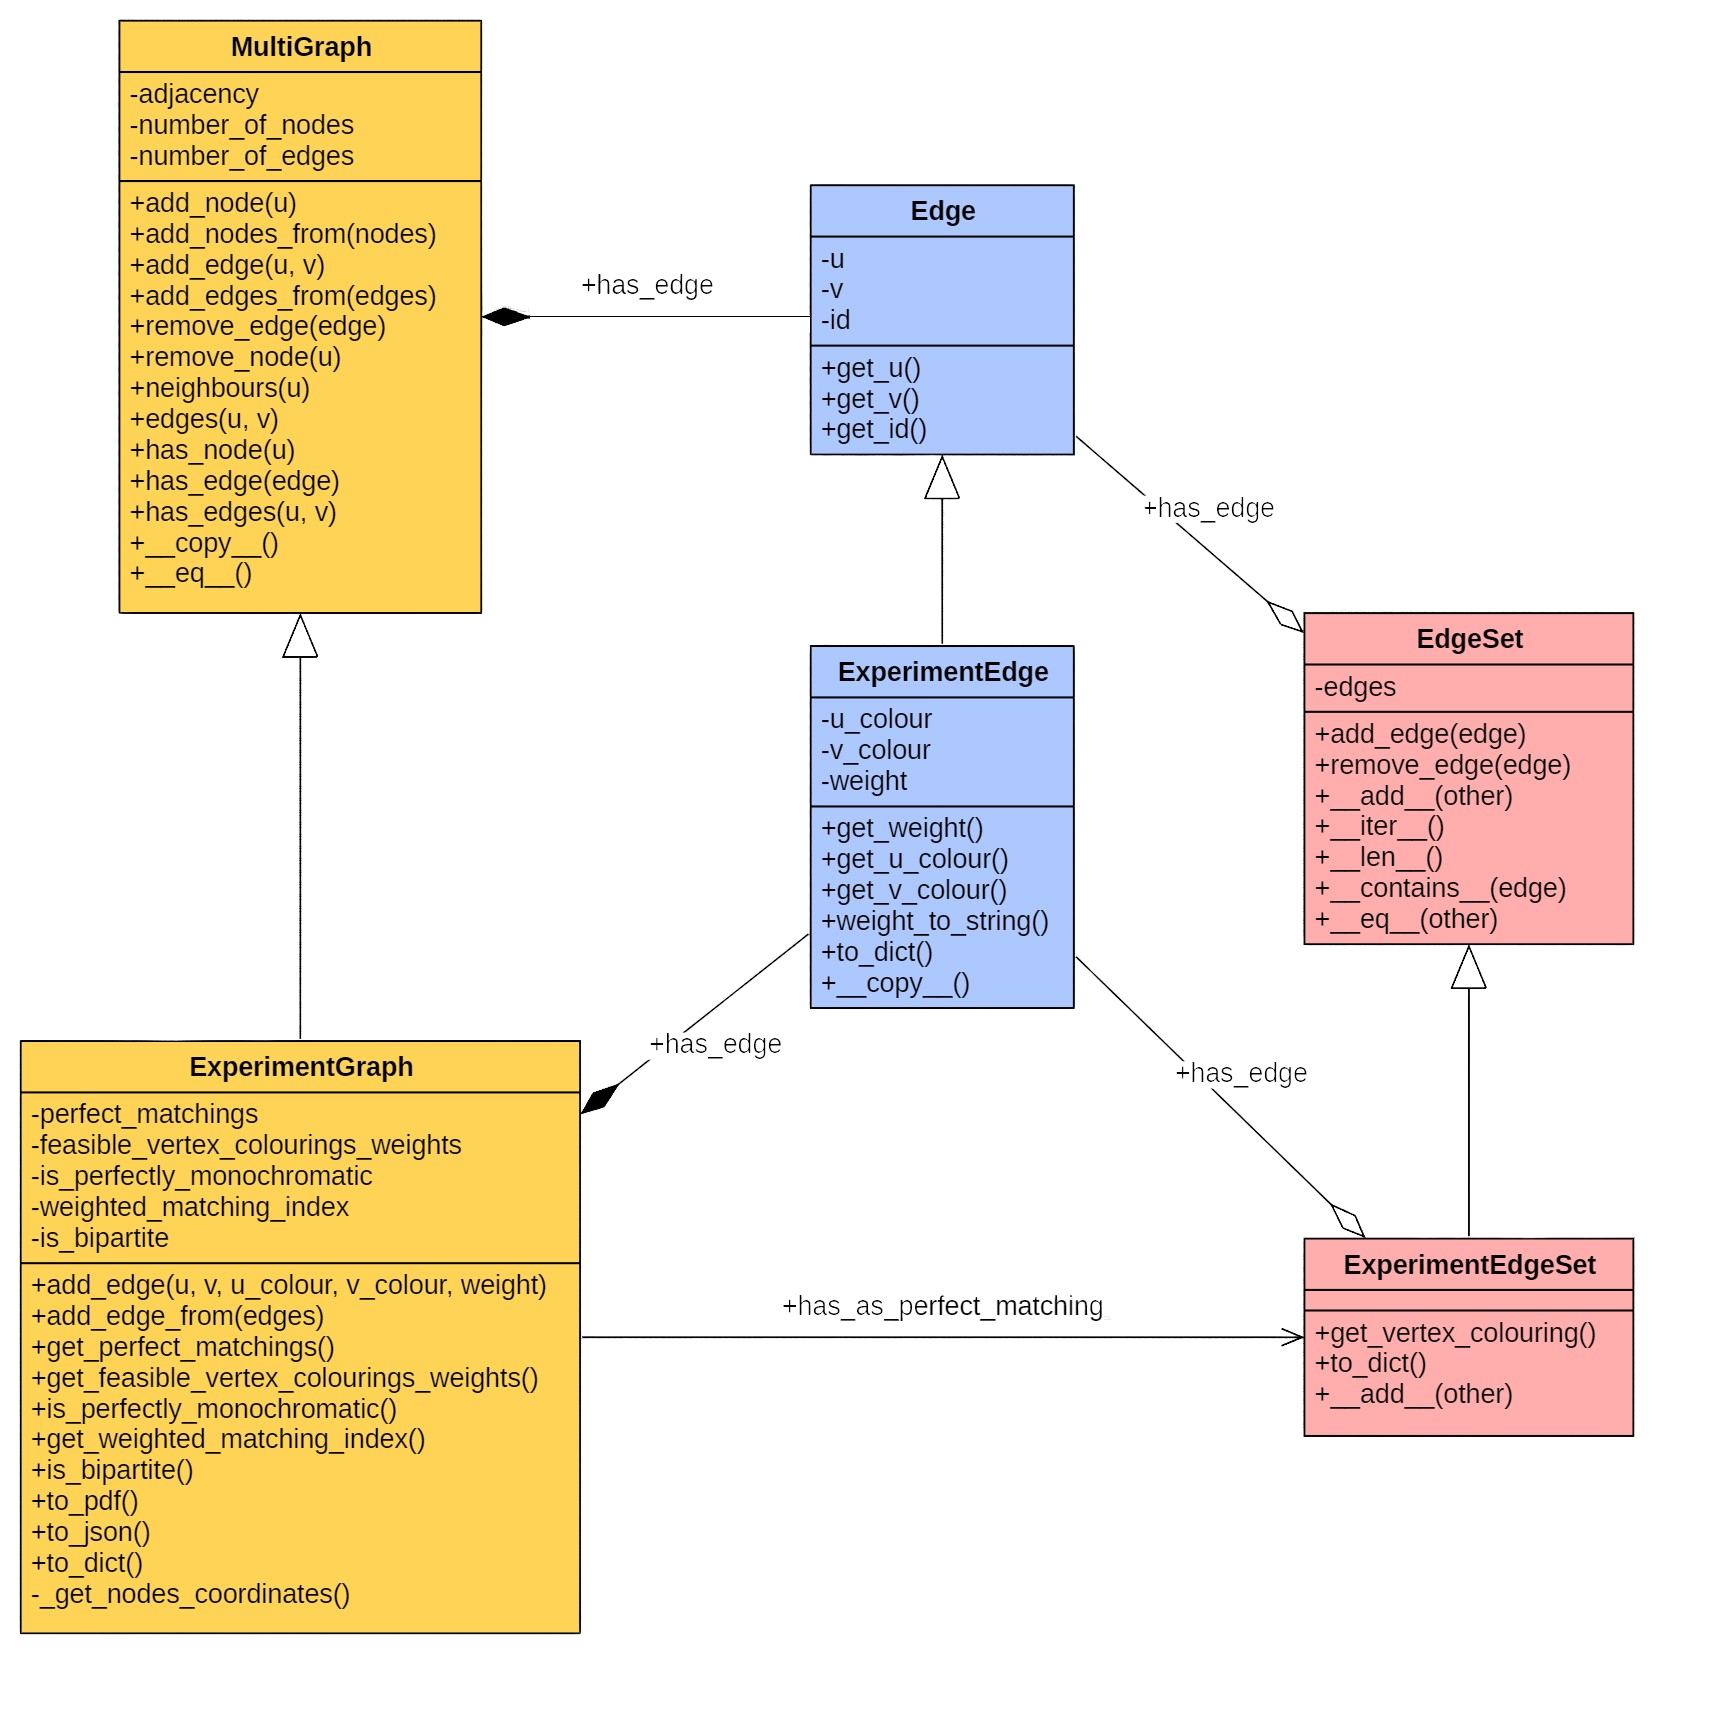
\includegraphics[scale=0.25]{figures/new_results/egpi/structure_diagram}
    \caption{Structure diagram of EGPI showing the important relations between the different implemented data structures. Most of the implemented methods of the program are shown in the diagram.}
    \label{fig:structure_diagram}
\end{figure}

Here is an exhaustive list of all non-trivial experiment graphs' properties we are interested to compute, and the algorithms we use in EGPI to do so.

\begin{enumerate}
    \item \textbf{Their perfect matchings:} to find all the perfect matchings of a graph, EGPI uses an algorithm written in pseudocode in algorithm~\ref{alg:perfect_matchings}.

        \begin{algorithm}
            \caption{Find all perfect matchings of an experiment graph $G$}
            \label{alg:perfect_matchings}
            \begin{algorithmic}
                \Require $G$ is an experiment graph
                \If{$G$ has no node}
                    \State The only perfect matching is $\varnothing$
                \ElsIf
                        {$G$ has nodes}
                    \State $PMs$ $\gets$ empty list
                    \State choose a random node $u \in V(G)$
                    \ForAll{$v \in$ neighbours of $u$}
                        \State $subPMs \gets$ all perfect matchings of $G$ without $u$ and $v$
                        \ForAll{$subPM \in subPMs$}
                            \ForAll{$e \in$ edges between $u$ and $v$}
                                \State add $subPM \cup e$ to $PMs$
                            \EndFor
                        \EndFor
                    \EndFor
                \EndIf
                \State \Return PMs
            \end{algorithmic}
        \end{algorithm}

        \paragraph{Complexity of algorithm \ref{alg:perfect_matchings}:} let $G_k^w$ be an experiment graph with $n_v$ vertices and $n_e$ edges.
        Let's introduce some notations.

        \begin{itemize}
            \item $\mu_d(n_v, n_e) = \frac{2 \cdot n_e}{n_v}$ is the expected degree of each vertex in average.
            \item $\mu_e(n_v, n_e) = \frac{n_e}{\left(\frac{n_v(n_v-1)}{2}\right)} = \frac{2n_e}{n_v(n_v-1)}$ is the average number of edges between $2$ defined nodes.
            \item $\mu_n(n_v, n_e) = \frac{\mu_d(n_v, n_e)}{n_v-1} = \frac{2 \cdot n_e}{n_v(n_v-1)}$ is the average neighbours' number of a node.
            \item $\mu_N(n_v)$ is the expected number of perfect matchings.
        \end{itemize}

        Let $T(n)$ denote the number of operations needed to run algorithm~\ref{alg:perfect_matchings} on $G_k^w$, and $N(n)$ be the number of perfect matchings of $G_k^w$.
        Using the recursion of the algorithm, it is clear that
        \begin{center}
            $\left\{ \begin{array}{r c l}
                T(0) & = & \mathcal{O}(1) \\
                T(n) & = & \mu_n(n_v, n_e) \cdot \left( T(n_v - 2) + \mu_N(n_v) \cdot \mu_e(n_v, n_e) \right)
            \end{array}\right.$
        \end{center}

        If $N(n_v) \cdot \mu_e(n_v, n_e) \ll T(n_v)$, (which is the case, since $T(n)$ grows exponentially as we will see), the equation can be simplified.
        \begin{center}
            $\left\{\begin{array}{r c l}
                        T(0) & = & \mathcal{O}(1)                            \\
                        T(n) & = & \mu_n(n_v, n_e) \cdot T(n_v - 2)          \\
                        & = & \frac{2 \cdot n_e}{n_v(n_v-1)} T(n_v - 2)      \\
            \end{array}\right.$
        \end{center}

    \item \textbf{The weights of their feasible vertex colourings:} according to their definition~\ref{def:feasible_vertex_colouring}, finding the feasible vertex colourings of an experiment graph requires to find their perfect matchings.
        The next steps to find them and their weights are simpler and are described in algorithm~\ref{alg:feasible_vertex_colourings}.

        \begin{algorithm}
            \caption{Find all feasible vertex colourings of an experiment graph $G_k^w$}
            \label{alg:feasible_vertex_colourings}
            \begin{algorithmic}
                \Require $G_k^w$ is an experiment graph
                \State $PMs \gets$ all perfect matchings of $G_k^w$
                \State $FVCs \gets$ empty Python dictionary
                \ForAll{$PM \in PMs$}
                    \State $FVC \gets$ feasible vertex colouring induced by $PM$
                    \State $w \gets$ weight of $PM$
                    \State $FVCs[FVC] \gets w$
                \EndFor
                \State \Return $FVCs$
            \end{algorithmic}
        \end{algorithm}

        The hardest step of this algorithm is to find all the perfect matchings of $G$.
        Therefore, the complexity of this algorithm is the same as the one of algorithm~\ref{alg:perfect_matchings}.

    \item \textbf{If the graph is perfectly monochromatic:} by definition~\ref{def:perfectly_monochromatic_graph}, finding if an experiment graph is perfectly monochromatic or not just requires to look at all its feasible vertex colourings.
        This is done in algorithm~\ref{alg:perfectly_monochromatic}.

        \begin{algorithm}
            \caption{Check if an experiment graph $G_k^w$ is perfectly monochromatic}
            \label{alg:perfectly_monochromatic}
            \begin{algorithmic}
                \Require $G_k^w$ is an experiment graph
                \State $FVCs \gets$ all feasible vertex colourings of $G$
                \State $isPM \gets$ True
                \ForAll{$FVC \in FVCs$}
                    \If{FVC is monochromatic and $w(FVC) \neq 1$}
                        \State $isPM \gets$ False
                    \ElsIf{FVC is not monochromatic and $w(FVC) \neq 0$}
                        \State $isPM \gets$ False
                    \EndIf
                \EndFor
                \State \Return $isPM$
            \end{algorithmic}
        \end{algorithm}

        The only hard step of this algorithm is to find all the feasible vertex colourings of $G$.
        Therefore, the complexity of this algorithm is the same as the one of algorithm~\ref{alg:feasible_vertex_colourings}.

    \item \textbf{The weighted matching index of the graph:} defined in definition~\ref{def:weighted_matching_index}, the weighted matching index of a perfectly monochromatic experiment graph is the number of monochromatic feasible vertex colourings in this graph.
        If the graph is not perfectly monochromatic, the weighted matching index is $0$ by definition.
        EGPI uses the algorithm~\ref{alg:weighted_matching_index} to compute the weighted matching index of a graph.
        \begin{algorithm}
            \caption{Compute the weighted matching index of an experiment graph $G_k^w$}
            \label{alg:weighted_matching_index}
            \begin{algorithmic}
                \Require $G_k^w$ is an experiment graph
                \State $FVCs \gets$ all feasible vertex colourings of $G_k^w$
                \State $isPM \gets$ is $G_k^w$ perfectly monochromatic ?
                \If{$isPM$}
                    \State $c \gets 0$
                    \ForAll{$FVC \in FVCs$}
                        \If{$w(FVC) = 1$}
                            \State $c \gets c + 1$
                        \EndIf
                    \EndFor
                    \State \Return $c$
                \Else
                    \State \Return $0$
                \EndIf
            \end{algorithmic}
        \end{algorithm}

    \item \textbf{If the graph is bipartite:} finding if a graph is bipartite or not is a well-known problem in graph theory.
        EGPI uses an algorithm based on the breadth-first search to find if a graph is bipartite or not.
        The algorithm is written in algorithm~\ref{alg:bipartite}.
        \begin{algorithm}
            \caption{Check if an experiment graph $G_k^w$ is bipartite}
            \label{alg:bipartite}
            \begin{algorithmic}
                \Require $G_k^w$ is an experiment graph
                \State $Q \gets$ empty queue
                \State add $v_0 \in V(G_k^w)$ to $Q$
                \State colour of $v_0 \gets$ red
                \State $isBipartite \gets$ True
                \While{$Q$ is not empty}
                    \State $u \gets$ pop $Q$
                    \ForAll{$v \in$ neighbours of $u$}
                        \If{colour of $v$ is not defined}
                            \State colour of $v \gets$ opposite colour of $u$
                            \State add $v$ to $Q$
                        \ElsIf{colour of $v$ is the same as colour of $u$}
                            \State $isBipartite \gets$ False
                        \EndIf
                    \EndFor
                \EndWhile
                \State \Return $isBipartite$
            \end{algorithmic}
        \end{algorithm}

        This algorithm is a greedy algorithm. It visits all the nodes of $G_k^w$.
        Therefore, its complexity is $\mathcal{O}(n_v)$, where $n_v$ is the number of vertices of $G_k^w$.

\end{enumerate}


\subsection{Limitations of EGPI}
\label{subsec:EGPI_limitations}

EGPI offers a pretty quick way to generate experiment graphs and compute their weighted matching index.
Then, it may be tempting to use it to prove the conjecture in some very restrained cases by generating and testing every possible experiment graph that respects some properties.
While this idea is theoretically possible, the user must be aware that he is extremely limited by the computational time of such an algorithm.
Indeed, the number of possible graphs grows exponentially with their degrees of freedom.\\

Let's consider a quick and simple example by trying to prove experimentally the following conjecture.

\begin{conjecture}
    \label{con:krenn_6}
    Let $G_k^w$ be a non-redundant experiment graph of size $n = 6$ vertices, and let say that, for all edge $e \in E(G)$,
    \begin{center}
        $\left\{\begin{array}{l l}
            Re(w(e)) & \in \{-1, 0, 1\} \\
            Im(w(e)) & \in \{-1, 0, 1\} \\
            w(e)     & \neq 0          \\
        \end{array}\right.$
    \end{center}
    Then, the weighted matching index $\Tilde{c}(G, k, w) \leq 2$.
\end{conjecture}

One way to prove the conjecture\ref{con:krenn_6} is to use a brute force algorithm that generates every possible graph respecting the pre-conditions of the conjecture~\ref{con:krenn_6} with bicoloured edges that can take their colours in $3$ defined colours $(r, g, b)$, and check their weighted matching index.
If none of their matching index is $3$, then the conjecture is true.
Unfortunately, this is not possible because of the following observation.\\

\begin{observation}
    Let $G_k^w$ be an experiment graph that has $n$ vertices, and let say that, for all edge $e = (u, v) \in E(G)$, the edge can have a value different from $0$ chosen among $W$ different values.
    Furthermore, $k(e, u)$ and $k(e, v)$ are chosen among $K$ different colours.
    At last, $\forall e' = (u, v), k(e') \neq k(e)$.
    Then, the number of different possible graphs that $G_k^w$, denoted $N_{graphs}$, is

    \begin{center}
        $N_{graphs} = (1 + W)^{\left(\frac{K^2 \cdot n \cdot (n-1)}{2}\right)}$
    \end{center}
\end{observation}


\begin{proof}
    Indeed, each edge $e$ is characterized by the following properties.
    \begin{itemize}
        \item It has a position $\{u, v\}$, that can take $\frac{n \cdot (n -1)}{2}$ different values.
        \item It has $2$ colours, one at each of its endpoint, that can take $K$ different values.
            Then, in total, there are $K^2$ different ways to bicolour it.
        \item It has a complex weight that can have $W$ different value.
    \end{itemize}

    A first observation is that the maximum number of edges between $2$ different nodes of $G$ is $K^2$.
    Indeed, more edges would imply that $2$ edges at least would have the same positions and colours, which is forbidden.\\

    Then, we observe that there are $W^x$ possibilities to assign weights to an edge set of size $x$.
    Using these $2$ last observations, it is possible to compute the number of different weighted bicoloured edges sets between $2$ defined nodes $u$ and $v$.
    Let's denote this number $N_{edges}$.

    \begin{center}
        $\begin{array}{r c l}
             N_{edges} & = & {K^2 \choose 0} W^0 + {K^2 \choose 1} W^1 + {K^2 \choose 2} W^2 + \cdots + {K^2 \choose K^2} W^{K^2} \\
                       & = & \sum\limits_{x=0}^{K^2} {K^2 \choose x} W^x
        \end{array}$
    \end{center}

    It is possible to simplify this expression by using the binomial theorem. \cite{wikipediaBinomialTheorem}

    \begin{center}
        $\begin{array}{r c l}
             N_{edges} & = & \sum\limits_{x=0}^{K^2} {K^2 \choose x} W^x               \\
                       & = & \sum\limits_{x=0}^{K^2} {K^2 \choose x} 1^{(K^2 - x)} W^x \\
                       & = & (1 + W)^{K^2}
        \end{array}$
    \end{center}

    Having this number, it is easy to find the number $N_{graphs}$ of possible experiment graphs.
    Indeed, we just have to choose one of the possible combinations of weighted bicoloured edges between $2$ defined nodes for each possible pair of nodes.
    The number of possible pair of nodes is $\frac{n \cdot (n-1)}{2}$.
    Therefore :

    \begin{center}
        $\begin{array}{r c l}
             N_{graphs} & = & N_{edges} ^ {\frac{n \cdot (n-1)}{2}}                  \\
                        & = & \left((1 + W)^{K^2}\right)^{\frac{n \cdot (n-1)}{2}}   \\
                        & = & (1 + W)^{\left({K^2} \cdot \frac{n \cdot (n-1)}{2}\right)} \\
        \end{array}$
    \end{center}
\end{proof}

Returning to conjecture~\ref{con:krenn_6}, let's compute as an example the number of graphs needed to verify to prove it by a brute force algorithm.
The graphs described in conjecture~\ref{con:krenn_6} have $n = 6$ vertices, $K = 3$ different possible colours per edge's endpoint, and $W = 8$ possible weights different from $0$.
Therefore, in this case,

\begin{center}
    $\begin{array}{r c l}
         N_{graphs} & = & (1 + W)^{\left(\frac{K^2 \cdot n \cdot (n-1)}{2}\right)} \\
                    & = & (1 + 8)^{\left(\frac{3^2 \cdot 6 \cdot (6-1)}{2}\right)} \\
                    & = & 9^{270}
    \end{array}$
\end{center}

This number is absurdly big, and it is totally impossible to imagine being able to generate all of those graphs on a classical computer and compute their matching index, no matter of how efficient this operation is.
Therefore, conjecture~\ref{con:krenn_6} cannot be solved by using a brute force algorithm, even if the graphs it is about are tiny and restricted compared to the space of all experiment graphs possible.


\subsection{Realized experiments with EGPI}
\label{subsec:realized_experiments}

In this section, I present some of the experiments I realized with EGPI. The goal of these experiments was to find interesting properties of experiment graphs, and to try to find a counter-example to the Krenn's conjecture.\\

\subsubsection{Research for counter-examples}

The first experiment I realized with EGPI was to try to find a counter-example to the Krenn's conjecture.
To do so, I performed three different random experiment graphs research processes, defined in definition~\ref{def:random_experiment_graphs_research_process}.
Each of these processes generated $10^7$ candidate graphs (defined in definition) with the following properties.

\begin{itemize}
    \item The possible colours of the edges were $L_{colours} = \{red, green, blue\}$.
    \item The possible complex weights of the edges were $L_{weights} = \{-1, 1, -i, i\}$.
    \item The complexity bound was an integer $b$ varying between $1$ and $6$.
        This choice was motivated by the fact that small and big complexity bounds have both their own interests.
        Indeed, small complexity bounds result in a smaller number of possible generated graphs, which increases the chance of finding a perfectly monochromatic graph in this space if it exists.
        This is experimentally verified in the next experiment.
        On the other hand, assuming that the Krenn's conjecture is false, the counter-examples to it might be very complex and impossible to generate with small complexity bounds.
\end{itemize}

The $3$ experiments generated graphs of size $n=6$, $n=8$ and $n=10$ vertices respectively.
On all the $30$ millions generated candidate graphs, none of them was perfectly monochromatic.
This result is a new argument in favour of the Krenn's conjecture, at least for graphs that have less than $10$ vertices.
Nevertheless, it does not constitute a proof of it in any case, and I encourage future researchers to continue looking for counterexamples to it alongside their researches (by using EGPI or any other method). \\


\subsubsection{Research for perfectly monochromatic graphs with a weighted matching index of $2$}

The second experiment I realized with EGPI was to try to find perfectly monochromatic graphs that have a weighted matching index of $2$.
These graphs are authorized by the Krenn's conjecture, and their properties are interesting to study.
Indeed, understanding better the structure of these graphs might help researchers to find new ideas in their seek for a proof to the conjecture.\\

But this is not the main and only interest of the experiment.
Exploring this class of experiment graphs is a great way to test the different functionalities of EGPI, and to experimentally check the impact of the different parameters of the program.
Using the following parameters,

\begin{itemize}
    \item The number of explored candidate graphs is $m = 10^6$.
    \item The possible colours of the edges were $L_{colours} = \{red, green\}$.
    \item The possible complex weights of the edges were $L_{weights} = \{-1, 1, -i, i\}$.
    \item The complexity bound was an integer $b$ varying between $1$ and $6$.
\end{itemize}

In three different random experiment graphs research processes generating graphs of size $n=6$, $n=8$ and $n=10$ vertices respectively, I got results summarized in figure~\ref{fig:results-experiment}.

\begin{figure}[H]
    \centering
    \begin{tabular}{ |p{1cm}||p{2cm}|p{2cm}|p{2cm}|p{2cm}|p{2cm}|p{2cm}|  }
        \hline
        \multicolumn{7}{|c|}{Results of the experiment} \\
        \hline
        $n$ & $b = 1$ & $b = 2$ & $b = 3$ & $b = 4$ & $b = 5$ & total \\
        \hline
        $6 $ & $199$ & $68$ & $9$ & $0$ & $0$ & $276$ \\
        $8 $ & $66$  & $0$  & $1$ & $0$ & $0$ & $67$   \\
        $10$ & $13$  & $0$  & $0$ & $0$ & $0$ & $13$  \\
        \hline
    \end{tabular}
    \caption{Results of $3$ different random experiment graphs research process with $n=6$, $n=8$ and $n=10$ respectively.}
    \label{fig:results-experiment}
\end{figure}

From the results in figure~\ref{fig:results-experiment}, we can do the following observations.
Firstly, it is a lot harder to find perfectly monochromatic graphs in these conditions when their size is bigger.
This can be explained by the fact that the number of possible graphs grows exponentially with the number of vertices.
Secondly, the complexity bound has a big impact on the number of found graphs.
A higher complexity bound results in a smaller number of found graphs.
This was expected, since the graphs generated with a higher complexity bound have higher chances to have more edges and perfect matchings.
The probability that all the randomly generated edges and perfect matchings together satisfy the definition~\ref{def:perfectly_monochromatic_graph} are small.\\

However, I am surprised that, when $n=8$, a graph was found with $b=3$ and none was found with $b=2$.
